%----------------------------------------------------------------------------------------
%	PACKAGES AND OTHER DOCUMENT CONFIGURATIONS
%----------------------------------------------------------------------------------------

\documentclass{article} % paper and 12pt font size

\newcommand\tab[1][1cm]{\hspace*{#1}}

\usepackage{amsmath,amsfonts,amsthm} % Math packages
\usepackage{fancyhdr}
\usepackage[catalan]{babel}
\usepackage[utf8]{inputenc}
\usepackage[T1]{fontenc}
\usepackage{color}
\usepackage{textcomp}
\usepackage{graphicx}
\usepackage{float}
\usepackage{listings}
\usepackage{enumitem}
\usepackage{textgreek}
\graphicspath{ {img/} }
\setlength\parindent{0pt} % Removes all indentation from paragraphs - comment this line for an assignment with lots of text

\pagestyle{fancy}
\fancyhf{}
\lhead{PAC1 - Aprenentatge computacional}
\rhead{Jordi Alvaro Arqués}
\cfoot{\thepage}

\begin{document}


\section{Exercici 1}

En aquest exercici haureu de mirar si es possible categoritzar l'arxiu petit de dades (small.csv). La darrera columna en aquest arxiu denota la classe. En particular, se us demana:
\begin{enumerate}
	\item Efectueu, si és necessari, el tractament previ de les dades. Justifiqueu totes les decisions que prengueu.
\end{enumerate}
{\color{blue}
	Ens proporcionen un arxiu amb dades relacionat amb vins:\\

	{\fontfamily{pcr}\selectfont\small
	\begin{tabular}{r r r r r r}
	 	ALCOHOL & ASH & MAGNESIUM & PHENOLS & COLOR & CLASS \\ \hline
		14.23 & 2.43 & 127 & 2.80 & 5.64 & 0 \\
		12.42 & 2.73 & 102 & 2.20 & 2.08 & 1 \\
		12.22 & 1.94 & 92  & 2.36 & 2.70 & 1 \\
		14.06 & 2.61 & 121 & 2.60 & 5.05 & 0 \\
		11.96 & 2.30 & 101 & 3.38 & 3.21 & 1 \\
		13.30 & 2.14 & 94  & 2.40 & 3.95 & 0 \\
		13.56 & 2.31 & 117 & 3.15 & 6.13 & 0 \\
		12.37 & 1.36 & 88  & 1.98 & 1.95 & 1 \\
	\end{tabular}
	} \\

	No hi ha valors absents, per tant, no els hem de tractar. Pel que fa als atributs, veiem que són numèrics i, tal i com es recomana al llibre de teoria de l'assignatura per al cas de valors numèrics, decidim aplicar estandardització per tal de normalitzar-los. A continuació, calcularem els promitjos i les desviacions estàndard.\\

	Per la característica "Alcohol" (ho marcarem amb el subíndex A), tenim el següent:

	\[mitjana_{A} = E(X_{A}) = \frac{1}{N}\sum\limits_{i=1}^N x_i\]
	\[mitjana_{A} = \frac{14.23 + 12.42 + 12.22 + 14.06 + 11.96 + 13.30 + 13.56 + 12.37}{8} = \frac{104.12}{8} = 13.02\]
	
	\[\sigma_{A} = \sqrt{\frac{1}{N}\sum\limits_{i=1}^N (x_i-E(X))^2}\]
	{\selectfont\tiny
	\[\sigma = \sqrt{\frac{(14.23-13.02)^2 + (12.42-13.02)^2 + (12.22-13.02)^2 + (14.06-13.02)^2 + (11.96-13.02)^2 + (13.30-13.02)^2 + (13.56-13.02)^2 + (12.37-13.02)^2}{8}} \]
	}
	\[\sigma_{A} = \sqrt{\frac{5.46}{8}}=0.83 \]

	Si ho repetim per a totes les altres acarcterístiques, obtenim la taula següent: \\ 

	{\fontfamily{pcr}\selectfont\small
	\begin{tabular}{c | r r r r r}
		 & ALCOHOL & ASH & MAGNESIUM & PHENOLS & COLOR \\ \hline
		 Mitjana & 13.02 & 2.23 & 105.25 & 2.61 & 3.84 \\
		\textsigma & 0.83 & 0.40 & 13.64 & 0.45 & 1.51 \\
	\end{tabular}
	}
	\\

	Ara normalitzem mitjançant el procediment d'estandarització totes les característiques de cada exemple. Ho fem de la següent manera:

	\[v_{A}' = \frac{v_{A} - E(X_{A})}{\sigma_{A}}\]
	\[v_{A}' = \frac{14.23 - 13.02}{0.83} = 1.47\]


	i el resultat global del procés:\\

	{\fontfamily{pcr}\selectfont\small
	\begin{tabular}{r r r r r r}
	 	ALCOHOL & ASH & MAGNESIUM & PHENOLS & COLOR & CLASS \\ \hline
		 1.47 &  0.50 &  1.60 &  0.43 &  1.19 & 0 \\
		-0.72 &  1.25 & -0.24 & -0.92 & -1.16 & 1 \\
		-0.96 & -0.71 & -0.97 & -0.56 & -0.75 & 1 \\
		 1.26 &  0.95 &  1.16 & -0.02 &  0.80 & 0 \\
		-1.28 &  0.18 & -0.31 &  1.73 & -0.42 & 1 \\
		 0.34 & -0.22 & -0.83 & -0.47 &  0.07 & 0 \\
		 0.66 &  0.21 &  0.86 &  1.21 &  1.51 & 0 \\
		-0.78 & -2.16 & -1.27 & -1.41 & -1.25 & 1 \\
	\end{tabular}
	} \\

}
\begin{enumerate}[resume]
	\item Utilitzeu el k-means nítid per a categoritzar les dades de l'esmentat arxiu en dues categories, ignorant les columnes no pertinents. Quin és el nivell de precisió\footnote{Per a calcular la precisió heu de comparar la categoria resultant per cada exemple amb la seva classe (última columna de l’arxiu).} del resultat?
\end{enumerate}
{\color{blue}
	Apliquem el k-means nítid amb la distància euclídea i dues categories a totes les columnes excepte l'última (classe). \\

	Hem seleccionat els dos primers exemples com a centroides inicials. Calculem les distàncies euclídees entre els centroides i tots els exemples. Distància entre l'exemple "i" i el centroide "j" \\

	\[d_{X_iC_j} = \sqrt{\sum\limits_{k=1}^N (x_{ik}-c_{jk})^2}\]

	La taula de distàncies euclídees seria la següent: \\

	{\fontfamily{pcr}\selectfont\small
	\begin{tabular}{r r r}
	 	          & Centroide 1 & Centroide 2 \\ \hline
		Exemple 3 & 4,33        & 2,18 \\
		Exemple 4 & 0,89        & 3,26 \\
		Exemple 5 & 3,94        & 3,00 \\
		Exemple 6 & 3,11        & 2,31 \\
		Exemple 7 & 1,42        & 3,99 \\
		Exemple 8 & 5,44        & 3,59 \\
	\end{tabular}
	} \\

	Els exemples pertanyen a la categoria del centroide més proper. Per tant, els exemples 3, 5, 6 i 8 pertanyen al centroide 2, metre que els exemples 4, i 7 pertanyen al centroide 1. Tornem a calcular els centroides fent la mitjana dels valors dels atributs (atribut a atribut) de tots els exemples de cada categoria. \\

	Exemple de recàlcul de la característica "Alcohol" del centroide 1 a partir dels exemples que hi pentanyen (1, 4 i 7): 

	\[m'_{A_{C_1}} = \frac{v_{A_1} + v_{A_4} + v_{A_7}}{3}= \frac{1.47 + 1.26 + 0.66}{3}=1.13\]


	Els nous centroides són: \\

	{\fontfamily{pcr}\selectfont\small
	\begin{tabular}{r r r r r}
		1,13  & 0,55  & 1,20  & 0,54  & 1,17 \\
		-0,68  & -0,33  & -0,72  & -0,32  & -0,70 \\
	\end{tabular}
	} \\
	

	Repetim aquest procés fins que no es produeixin canvis en les categories. Obtenim els centroides finals: \\

	{\fontfamily{pcr}\selectfont\small
	\begin{tabular}{r r r r r}
		1.13  & 0.55  & 1.20  & 0.54  & 1.17 \\
		-0.68 & -0.33 & -0.72 & -0.32 & -0.70 \\
	\end{tabular}
	} \\

	I com a categories finals:
	\begin{itemize}
		\item[] Cat. 1: \{1, 4, 7\}
		\item[] Cat. 2: \{2, 3, 5, 6, 8\}
	\end{itemize}

	Si assignem la classe "0" a la categoria 1 i la classe "1" a la categoria 2, obtenim una presició:

	\[presicio = \frac{3 + 4}{8} = 87.5\%\]

	El k-means depèn molt dels centroides inicials escollits. Si agafem com a centroides inicial els dos últims exemples obtenim els centroides: \\

	{\fontfamily{pcr}\selectfont\small
	\begin{tabular}{r r r r r}
		0.53  & 0.46  & 0.83  & 0.84  & 0.77 \\
		-0.53 & -0.46 & -0.83 & -0.84 & -0.77 \\
	\end{tabular}
	} \\

	I les categories:
	\begin{itemize}
		\item[] Cat. 1: \{1, 3, 6, 7\}
		\item[] Cat. 2: \{2, 4, 5, 8\}
	\end{itemize}

	Si assignem la classe "0" a la categoria 1 i la classe "1" a la categoria 2, obtenim una presició:

	\[presicio = \frac{3 + 3}{8} = 75\%\]

}
\begin{enumerate}[resume]
	\item Apliqueu l'algorisme PCA per a reduir la dimensionalitat del conjunt anterior conservant el 95\% de la variància. Utilitzeu el k-means nítid sobre el conjunt reduït de la mateixa forma que en l'apartat anterior. Comparau els resultats.  
\end{enumerate}
{\color{blue} \leftmargin=4in
	Apliquem el PCA sobre el conjunt de l'arxiu. Obtenim els percentatges de variàncies dels components principals: \\

	{\fontfamily{pcr}\selectfont\small
	\begin{tabular}{r r r r r}
		0.67 & 0.17 & 0.13 & 0.02 & 0.00 \\
	\end{tabular}
	} \\

	Si les acumulem: \\

	{\fontfamily{pcr}\selectfont\small
	\begin{tabular}{r r r r r}
		0.67 & 0.84 & 0.98 & 1.00 & 1.00 \\
	\end{tabular}
	} \\

	Per tant, veiem que només necessitem 3 components principals per tal de mantenir el 95\% de la variància de les dades inicials. Si apliquem la conversió, obtenim la següent taula (hem reduït 2 dimensions): \\

	{\fontfamily{pcr}\selectfont\small
	\begin{tabular}{r r r}
		-2.45 &  0.64 &  0.15 \\
		 0.89 & -0.21 & -1.87 \\
		 1.79 & -0.09 &  0.11 \\
		-1.94 &  0.66 & -0.51 \\
		 0.30 & -2.17 &  0.32 \\
		 0.48 &  0.55 &  0.12 \\
		-2.01 & -0.36 &  0.85 \\
		 2.94 &  0.98 &  0.82 \\
	\end{tabular}
	} \\

	No obstant, hem perdut el significat de cadascuna de les característiques. N'hi ha tres de noves que són una combinació lineal de les inicials, en base als vectors i valors propis que s'han obtingut mitjançant el PCA. \\

	Ara, apliquem el k-means com en l’exercici anterior. Els centroides obtinguts són: \\

	{\fontfamily{pcr}\selectfont\small
	\begin{tabular}{r r r r r}
		-0.07 &  0.03 &  0.33 \\
		 0.49 & -0.23 & -2.29 \\
	\end{tabular}
	} \\

	I les categories:

	\begin{itemize}
		\item[] Cat. 1: \{1, 3, 4, 5, 6, 7, 8\}
		\item[] Cat. 2: \{2\}
	\end{itemize}

	Si assignem la classe "0" a la categoria 1 i la classe "1" a la categoria 2, obtenim una presició:

	\[presicio = \frac{4 + 1}{8} = 62.5\%\]
}

\section{Exercici 2}
En aquest exercici haureu de categoritzar les dades amb el mètode aglomeratiu. En particular, heu de construir tres dendrogrames per al mateix conjunt de dades que a l'exercici anterior (small.csv) utilitzant la distància euclidia. Com a criteris d'aglomeració emprau el lligam simple per al primer dendrograma, el lligam complet per al segon i la mitja per al tercer. Calculeu les precisions de la mateixa forma que a l'exercici anterior.
\\

{\color{blue}
	El primer que hem de fer és calcular la matriu de distàncies. Aquestes distàncies les obtindrem de cada parell d'objectes aplicant la distància euclídea sobre els seus valors normalitzats. \\

	Exemple: 
	{\selectfont\small
	\[d_{12}=\sqrt{(1.47-(-0,72))^2 + (0.50-1.25)^2 + (1.60-(-0.24))^2 + (0.43-(-0.92))^2 + (1.19-(-1.16))^2}= 4.00715103\]
	}

	La taula final serà: \\

	{\fontfamily{pcr}\selectfont\small
	\begin{tabular}{r r r r r r r r}
		  & 1          & 2          & 3          & 4          & 5          & 6          & 7          \\
		2 & 4.00715103 &            &            &            &            &            &            \\
		3 & 4.32844563 & 2.17922355 &            &            &            &            &            \\
		4 & 0.88829168 & 3.25953547 & 3.8672903  &            &            &            &            \\
		5 & 3.94406769 & 3.00181717 & 2.58382633 & 3.7066599  &            &            &            \\
		6 & 3.11351311 & 2.3144805  & 1.63318294 & 2.61931048 & 2.84888626 &            &            \\
		7 & 1.41583999 & 3.98724559 & 3.88698778 & 1.74279261 & 3.0191097  & 2.83254301 &            \\
		8 & 5.44461898 & 3.59239709 & 1.78005594 & 5.08144139 & 4.14188606 & 2.80215184 & 5.16512108 \\
	\end{tabular}
	} \\

	A partir d’aquest moment començarem el procés iteratiu. El primer pas és mirar quina és la distància mínima. Veiem que és entre els exemples 1 i 4 (d = 0.88829168). Hem d’eliminar les entrades de la matriu dels dos exemples i afegir una nova entrada que els agrupi:\\

	{\fontfamily{pcr}\selectfont\small
	\begin{tabular}{r r r r r r r r}
		  & 1 + 4      & 2          & 3          & 5          & 6          & 7          \\
		2 &         -- &            &            &            &            &            \\
		3 &         -- & 2.17922355 &            &            &            &            \\
		5 &         -- & 3.00181717 & 2.58382633 &            &            &            \\
		6 &         -- & 2.3144805  & 1.63318294 & 2.84888626 &            &            \\
		7 &         -- & 3.98724559 & 3.88698778 & 3.0191097  & 2.83254301 &            \\
		8 &         -- & 3.59239709 & 1.78005594 & 4.14188606 & 2.80215184 & 5.16512108 \\
	\end{tabular}
	} \\

	En aquest punt hem d’afegir les distàncies corresponents al nou element. Aquí és on difereixen els tres mètodes: enllaç simple, complert i mitjana. Per a l’enllaç simple escollirem la distància mínima, per al complert la màxima i per l’últim la mitjana aritmètica de les distàncies. \\

	Simple: \(min(d_{1,i}, d_{4,i})\)


	{\fontfamily{pcr}\selectfont\small
	\begin{tabular}{r r r r r r r r}
		  & 1 + 4      & 2          & 3          & 5          & 6          & 7          \\
		2 & 3.25953547 &            &            &            &            &            \\
		3 & 3.8672903 & 2.17922355 &            &            &            &            \\
		5 & 3.7066599 & 3.00181717 & 2.58382633 &            &            &            \\
		6 & 2.61931048 & 2.3144805  & 1.63318294 & 2.84888626 &            &            \\
		7 & 1.41583999 & 3.98724559 & 3.88698778 & 3.0191097  & 2.83254301 &            \\
		8 & 5.08144139 & 3.59239709 & 1.78005594 & 4.14188606 & 2.80215184 & 5.16512108 \\
	\end{tabular}
	} \\

	Complert: \(max(d_{1,i}, d_{4,i})\)


	{\fontfamily{pcr}\selectfont\small
	\begin{tabular}{r r r r r r r r}
		  & 1 + 4      & 2          & 3          & 5          & 6          & 7          \\
		2 & 4.00715103 &            &            &            &            &            \\
		3 & 4.32844563 & 2.17922355 &            &            &            &            \\
		5 & 3.94406769 & 3.00181717 & 2.58382633 &            &            &            \\
		6 & 3.11351311 & 2.3144805  & 1.63318294 & 2.84888626 &            &            \\
		7 & 1.74279261 & 3.98724559 & 3.88698778 & 3.0191097  & 2.83254301 &            \\
		8 & 5.44461898 & 3.59239709 & 1.78005594 & 4.14188606 & 2.80215184 & 5.16512108 \\
	\end{tabular}
	} \\

	Mitjana: \(avg(d_{1,i}, d_{4,i})\)


	{\fontfamily{pcr}\selectfont\small
	\begin{tabular}{r r r r r r r r}
		  & 1 + 4      & 2          & 3          & 5          & 6          & 7          \\
		2 & 3.63334325 &            &            &            &            &            \\
		3 & 4.097867965 & 2.17922355 &            &            &            &            \\
		5 & 3.825363795 & 3.00181717 & 2.58382633 &            &            &            \\
		6 & 2.866411795 & 2.3144805  & 1.63318294 & 2.84888626 &            &            \\
		7 & 1.5793163 & 3.98724559 & 3.88698778 & 3.0191097  & 2.83254301 &            \\
		8 & 5.263030185 & 3.59239709 & 1.78005594 & 4.14188606 & 2.80215184 & 5.16512108 \\
	\end{tabular}
	} \\

	En aquest punt hem de tornar a començar amb el procés iteratiu que finalitzarà quan només quedin dos grups d’objectes. A continuació es mostren els dendrogrames i les agrupacions resultants per als tres mètodes: \\

	Agrupacions (mètode enllaç simple): 

	{\fontfamily{pcr}\selectfont\small
	\begin{tabular}{r}
		\{1, 4\} \\
		\{1, 4, 7\} \\
		\{3, 6\} \\
		\{3, 6, 8\} \\
		\{2, 3, 6, 8\} \\
        \{2, 3, 5, 6, 8\} \\
 		\{1, 2, 3, 4, 5, 6, 7, 8\} \\
	\end{tabular}
	} \\

	Dendograma (mètode enllaç simple):

	\begin{figure}[H]
		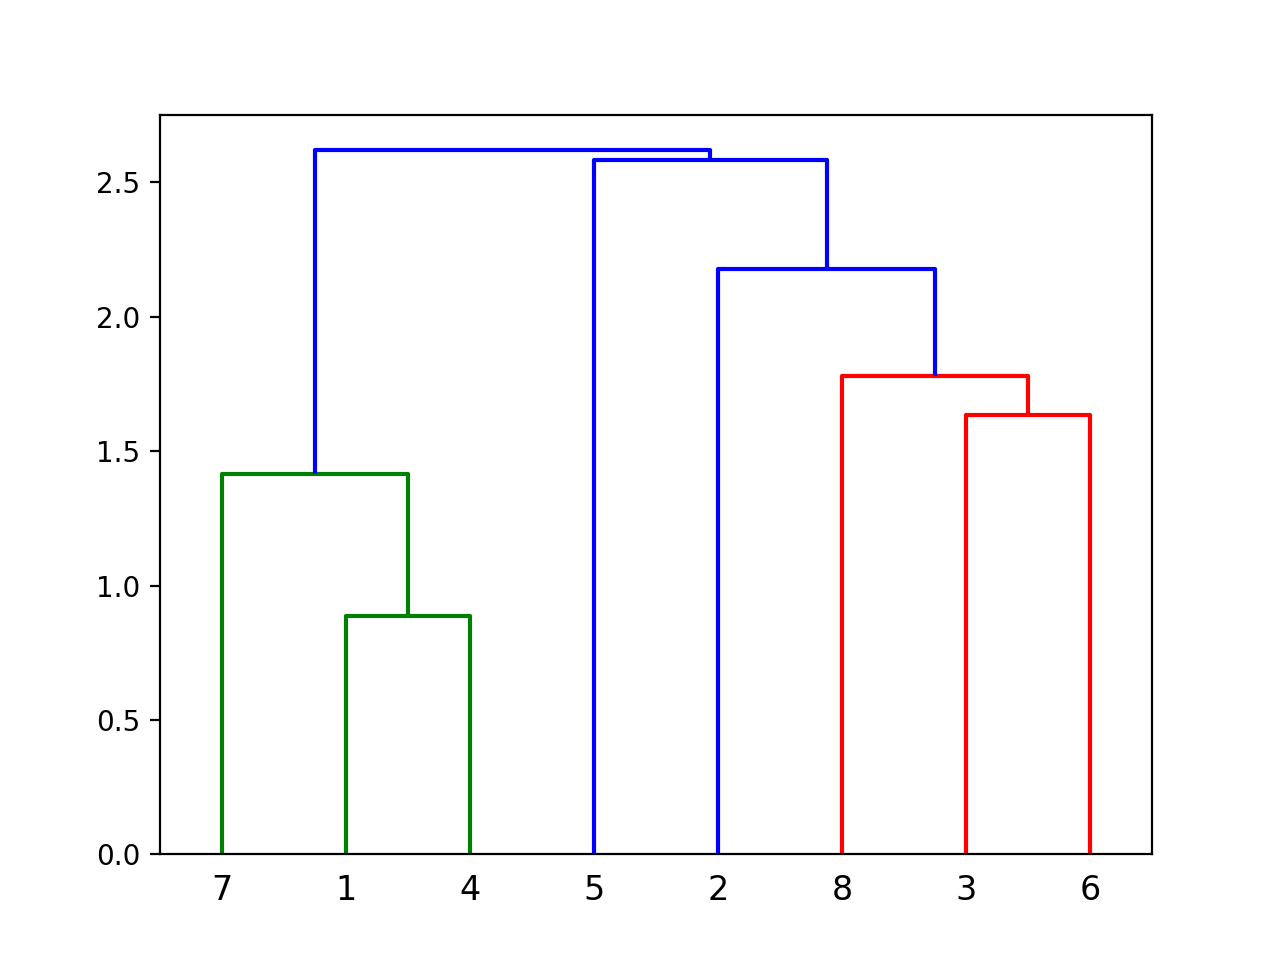
\includegraphics[width=10cm]{single}
		\centering
		\color{blue}
		\caption{Dendograma construït utilitzant el mètode \textbf{\textit{enllaç simple}}.}\label{visina8}
	\end{figure}

	Si considerem només 2 categories per l'ordre d'agrupació obtenim els grups:

	\begin{itemize}
		\item[] Cat. 1: \{1, 4, 7\}
		\item[] Cat. 2: \{2, 3, 5, 6, 8\}
	\end{itemize}

	Si assignem la classe "0" a la categoria 1 i la classe "1" a la categoria 2, obtenim una presició:

	\[presicio = \frac{3 + 4}{8} = 62.5\%\] \\

	Agrupacions (mètode enllaç complert):

	{\fontfamily{pcr}\selectfont\small
	\begin{tabular}{r}
		\{1, 4\} \\
		\{3, 6\} \\
		\{1, 4, 7\} \\
		\{2, 3, 6\} \\
		\{2, 3, 5, 6\} \\
        \{2, 3, 5, 6, 8\} \\
 		\{1, 2, 3, 4, 5, 6, 7, 8\} \\
	\end{tabular}
	} \\

	Dendograma (mètode enllaç complert):

	\begin{figure}[H]
		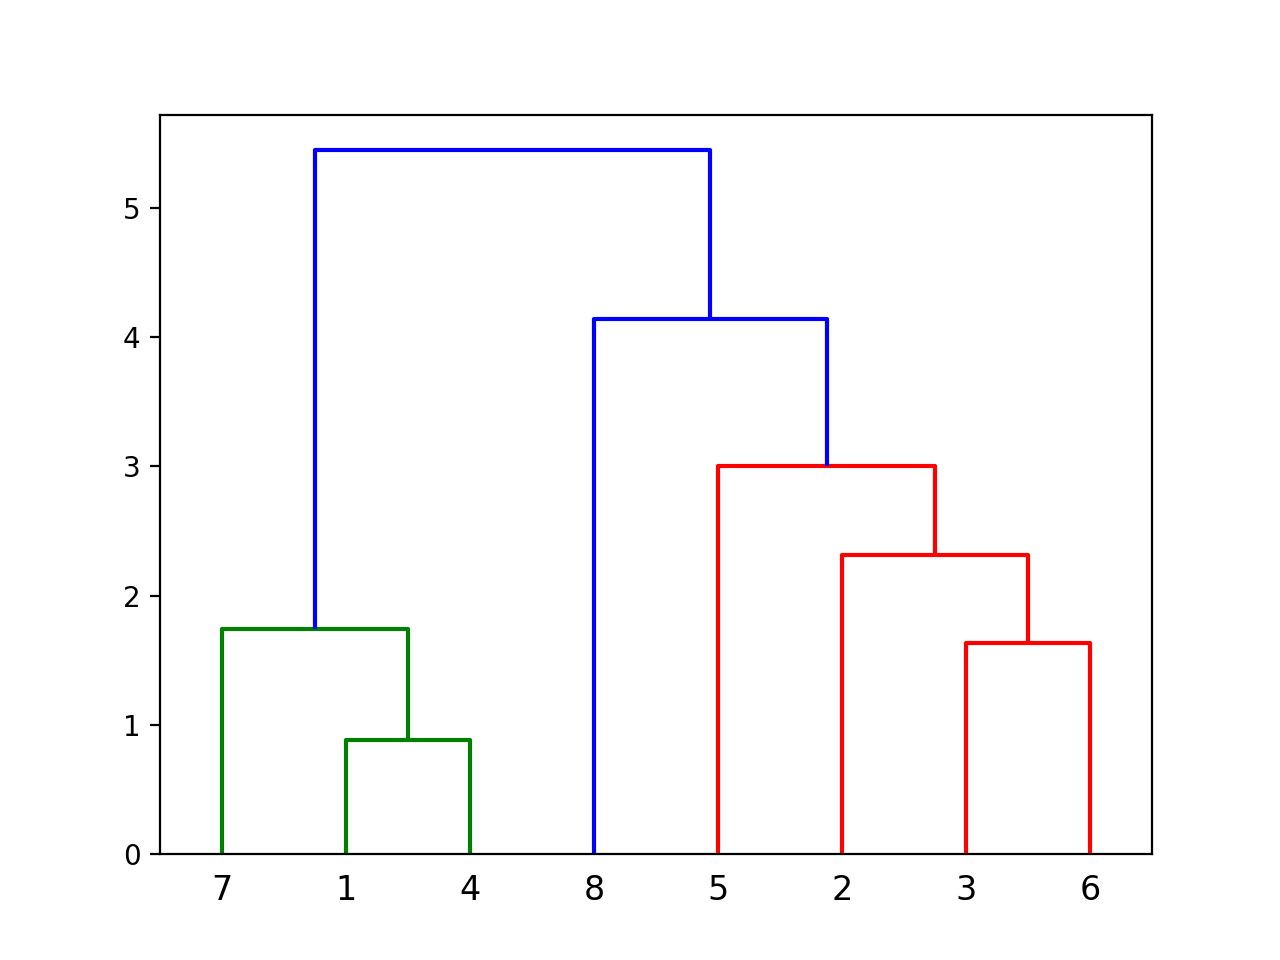
\includegraphics[width=10cm]{complete}
		\centering
		\color{blue}
		\caption{Dendograma construït utilitzant el mètode \textbf{\textit{enllaç complert}}.}\label{visina8}
	\end{figure}

	Si considerem només 2 categories per l'ordre d'agrupació obtenim els mateixos grups i precisió que amb el mètode anterior. \\


	Agrupacions (mètode enllaç mitjana): 

	{\fontfamily{pcr}\selectfont\small
	\begin{tabular}{r}
		\{1, 4\} \\
		\{1, 4, 7\} \\
		\{3, 6\} \\
		\{2, 3, 6\} \\
		\{2, 3, 6, 8\} \\
        \{2, 3, 5, 6, 8\} \\
 		\{1, 2, 3, 4, 5, 6, 7, 8\} \\
	\end{tabular}
	} \\

	Dendograma (mètode enllaç mitjana):

	\begin{figure}[H]
		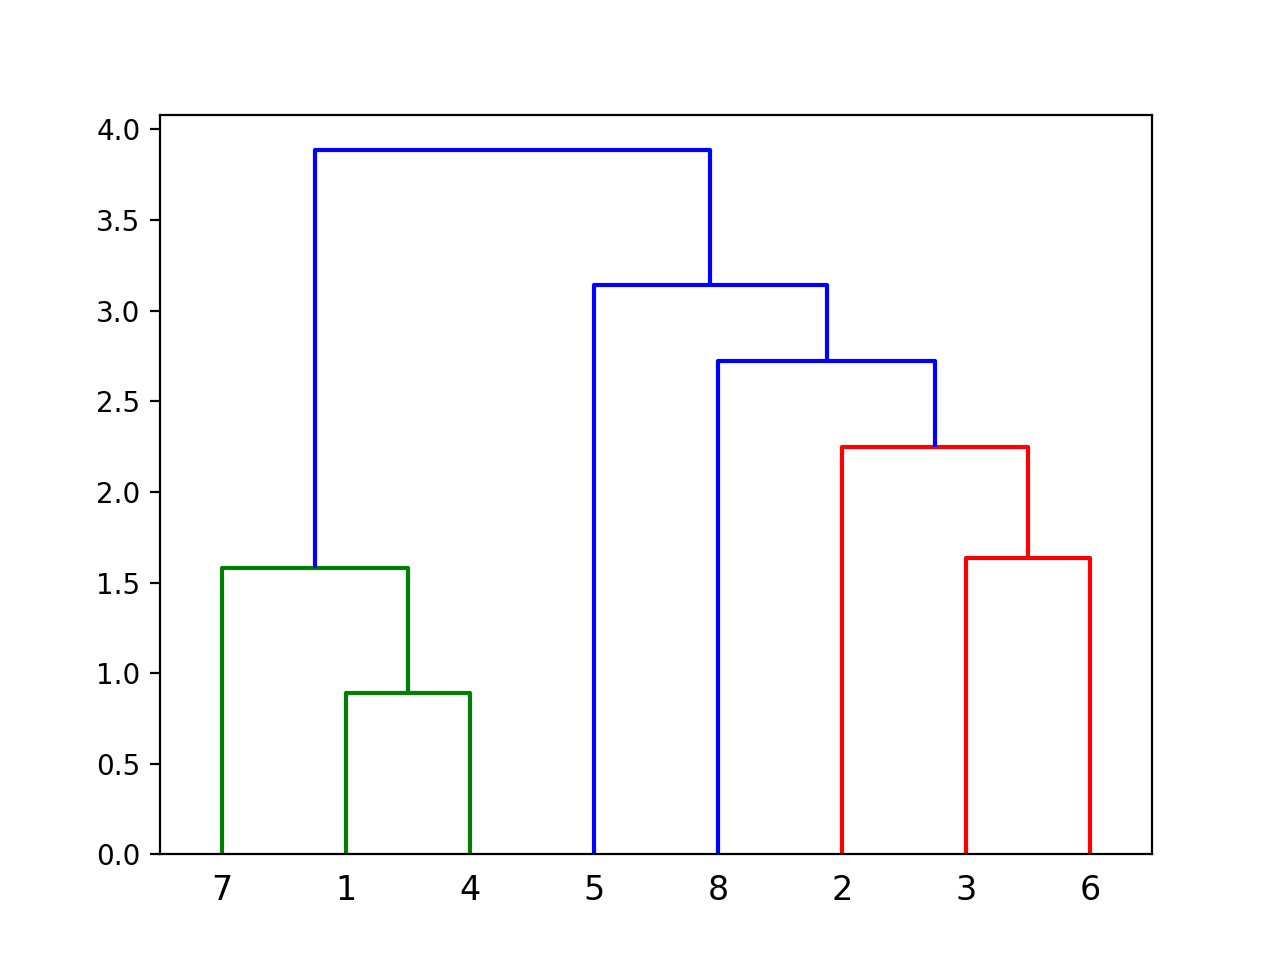
\includegraphics[width=10cm]{average}
		\centering
		\color{blue}
		\caption{Dendograma construït utilitzant el mètode \textbf{\textit{enllaç mitjana}}.}\label{visina8}
	\end{figure}

	Si considerem només 2 categories per l'ordre d'agrupació obtenim els mateixos grups i precisió que amb els mètodes anteriors.
}

\section{Exercici 3}
En aquest exercici haureu d'emprar unes biblioteques en Python per tal de categoritzar l'arxiu gran adjunt (wine.csv) en dues categories. La biblioteca s'anomena scikit-learn i la podeu descarregar i llegir-ne la documentació a la seva plana Web: \\

http://scikit-learn.org \\

En particular, se us demana que apliqueu, sobre les dades de l'arxiu esmentat, el mètode k-means (anomenat KMeans) amb dos criteris distints per a triar els centroides inicials i un altre mètode a escollir. Mostrau els resultats més destacables de cada categorització i calculau la precisió en cada cas. No heu d'adjuntar el codi, però sí heu de mostrar per a cada un dels tres casos (k-means amb el primer criteri, k-means amb el segon i mètode a escollir) la línia o línies que defineixen i parametritzen el categoritzador.
\\

{\color{blue}
	A l'exercici 1, el mètode k-means s'ha utilitzat predefinint els centroides inicials manualment (o bé els dos primers o bé els dos últims). No obstant, la documentació del mètode KMeans de la llibreria scikit ens dóna dues opcions més. La variable init permet els següents valors (a part de prefixar els centroides):
	\begin{itemize}
		\item 'k-means++'. Selecciona els centroides de forma intel·ligent per tal de minimitzar el temps de convergència.
		\item 'random'. Selecciona k observacions aleatòriament.
	\end{itemize}

	Tant si s'executa l'una com l'altra, en el cas que ens pertoca, obtenim els mateixos resultats. De fet, inclús provant de disminuir el número màxim d'iteracions en el pitjor cas ('random'), s'ha pogut comprovar que amb 3 iteracions n'hi ha suficient per a categoritzar les mostres amb un 93,84\% de precisió. \\

	Centroides: \\

	{\fontfamily{pcr}\selectfont\tiny
	\begin{tabular}{r r r r r r r r r r r r r}
		0.75 & -0.04 & 0.35 & -0.34 & 0.43 & 0.66& 0.70 & -0.41 & 0.32 & 0.72 & 0.07 & 0.42 & 0.77 \\
		-0.80 & 0.04 & -0.38 & 0.36 & -0.46 & -0.70 & -0.74 & 0.44 & -0.34 & -0.76 & -0.08 & -0.45 & -0.82 \\
	\end{tabular}
	} \\

	Categories:

	\begin{itemize}
		\item[] Cat. 1: \{1, 2, 3, 4, 5, 6, 7, 8, 9, 10, 11, 12, 13, 14, 15, 16, 17, 18, 19, 20, 21, 22, 23, 24, 25, 26, 27, 28, 29, 30, 31, 32, 33, 34, 35, 36, 37, 38, 39, 40, 41, 42, 43, 44, 45, 46, 47, 48, 49, 50, 51, 52, 53, 54, 55, 56, 57, 58, 59, 64, 67, 72, 74, 75, 96, 99, 122\}
		\item[] Cat. 2: \{60, 61, 62, 63, 65, 66, 68, 69, 70, 71, 73, 76, 77, 78, 79, 80, 81, 82, 83, 84, 85, 86, 87, 88, 89, 90, 91, 92, 93, 94, 95, 97, 98, 100, 101, 102, 103, 104, 105, 106, 107, 108, 109, 110, 111, 112, 113, 114, 115, 116, 117, 118, 119, 120, 121, 123, 124, 125, 126, 127, 128, 129, 130\}
	\end{itemize}

	I si assignem la classe "0"a la categoria 1 i la classe "1"a la categoria 2, obtenim una presició:

	\[presicio = 93.84\%\] \\

	Un altre mètode que s'ha provat és el Birch. Aquest mètode crea un estructura de dades en forma d'arbre. És planteja com una alternativa més eficient al k-means. Una altra cosa rellevant d'aquest algorisme és que també ens permet veure els centroides. A continuació, es mostra tota la informació obtinguda amb aquest mètode: \\

	Centroides: \\

	{\fontfamily{pcr}\selectfont\small
	\begin{tabular}{r r r r r r r r r r r r r}
		0.83 & -0.16 & 0.07 & -0.47 & 0.27 & -0.19 & 0.27 & 0.83 & 0.40 & -0.22 & 1.02 & -0.18 & 0.57 \\
		0.38 & -0.37 & 1.69 & -0.97 & 0.66 & 0.14 & 0.26 & 0.09 & -0.73 & 0.25 & 0.19 & -0.37 & 0.26 \\
	\end{tabular}
	} \\

	Categories:

	\begin{itemize}
		\item[] Cat. 1: \{1, 2, 3, 4, 5, 6, 7, 8, 9, 10, 11, 12, 13, 14, 15, 16, 17, 18, 19, 20, 21, 22, 23, 24, 25, 26, 27, 28, 29, 30, 31, 32, 33, 34, 35, 36, 37, 38, 39, 40, 41, 42, 43, 44, 45, 46, 47, 48, 49, 50, 51, 52, 53, 54, 55, 56, 57, 58, 59, 72, 74, 80, 111, 122, 123, 124, 125\}
		\item[] Cat. 2: \{60, 61, 62, 63, 64, 65, 66, 67, 68, 69, 70, 71, 73, 75, 76, 77, 78, 79, 81, 82, 83, 84, 85, 86, 87, 88, 89, 90, 91, 92, 93, 94, 95, 96, 97, 98, 99, 100, 101, 102, 103, 104, 105, 106, 107, 108, 109, 110, 112, 113, 114, 115, 116, 117, 118, 119, 120, 121, 126, 127, 128, 129, 130\}
	\end{itemize}

	I si assignem la classe "0"a la categoria 1 i la classe "1"a la categoria 2, obtenim una presició:

	\[presicio = 93.84\%\]
}

\section{Exercici 4}
Realitzau una valoració global comparant els mètodes dels exercicis anteriors i els resultats que n'heu obtingut. Redacteu unes conclusions globals. Els criteris de correcció de la PAC invaliden una A si tots els processos no estan ben justificats.
\\

{\color{blue}
	Per a mostres petites com als arxius small.csv, és important diferenciar entre la variància mostral i la poblacional. De totes formes, a efectes pràctics, per a mostres grans, la diferència és residual i l'efecte és mínim. \\

	L'estandarització és un bon sistema per a tractar dades numèriques i poder-les normalitzar de forma que puguem comparar i treballar més fàcilment amb les diferents característiques. \\

	Pel que fa a la tècnica d'extracció de característiques PCA, cal dir que és important quan saber usar-la. Pot ser realment molt útil en un entorn en el que tinguem un nombre molt gran de característiques, ja que ens permet reduir el nostre espai de valors, reduint també l'emmagatzematge i el cost computacional del procés d'aprenentatge tot mantenint uns límits de pèrdua d'informació (ho podem controlar a través de la variància tal i com s'ha vist a l'exercici 1). No obstant, un dels inconvenients és que perdem l'habilitat de poder intuir quines característiques són les que més afecten al sistema ja que, un cop aplicat el PCA, les noves característiques són combinacions lineals de les originals, sense un significat directe als atributs inicials. \\

	L'algorisme k-means depèn molt dels centroides inicials escollits. Hi ha vàries estratègies per escollir-los, ja sigui a l'atzar, a partir de la mitjana, etc. També es podria donar el cas extrem en que les nostres dades estiguessin separades en un grup molt gran i un altre de molt petit; llavors, si escollissim malament els centroides podria ser que no aconseguissim dividir bé l'espai i no arribar a categoritzar bé el grup petit (això no ho hem vist en aquesta pràctica). \\

	També s'ha pogut observar que amb poques dades, el k-means obté una precisió bastant baixa ja que no té una suficient quantitat de mostres per a poder aprendre i seleccionar les característiques importants. D'altra banda, quan s'ha augmentat el nombre de mostres de 8 a 130, ja s'han obtingut una precisió molt bona i constant. S'ha executat múltiples vegades el k-means amb 'random' per a escollir centroides aleatòriament i sempre s'ha obtingut la mateixa precisió. De fet, s'ha vist que amb 3 iteracions ja s'obtenia aquest valor. \\

	El mètode Burch ha mostrat uns valors molt similars al k-means. \\

	Pel que fa al scikit, cal dir que és una eina molt útil, pràctica, fàcil d'utilitzar i completa. Tot i que només en aquesta memòria només s'ha mostrat els resultats per al Birch, he pogut provar diferents algorismes (AgglomerativeClustering, DBSCAN, MeanShift). A més, la disponibilitat d'aquesta llibreria de poder ser utilitzada amb Python (i també amb la llibreria numpy), afegeix un potencial enorme a aquesta eina.
}

\end{document}